\graphicspath{{chapters/04/images/}}
\chapter{Approximation algorithms}

\section{Introduction}
Exact simulation of complex biological system is often to expensive due to their stochastic and multi scale nature.
These lead to the development of approximate algorithms, which improve the simulation efficiency by sacrificing their accuracy.
Multiple firings are coalesced and performed together in one simulation step with a huge speed up.
Approximate methods should be used because:

\begin{multicols}{2}
  \begin{itemize}
    \item It might be the only possible and feasible solution to solve a problem.
    \item reality is affected by error, so even when using exact stochastic simulation algorithms a small degree of approximation should be considered.
      A certain deal of error could aid in retrieving a more realistic result.
  \end{itemize}
\end{multicols}

In this case, each algorithm (Figure \ref{fig:SSA_tree}) approximates in a different way,  assuming different approximations.
Of the three main computational strategies presented here, there is one which is much more popular with respect to the others the $\tau$ leaping method.

\begin{figure}]H]
  \centering
  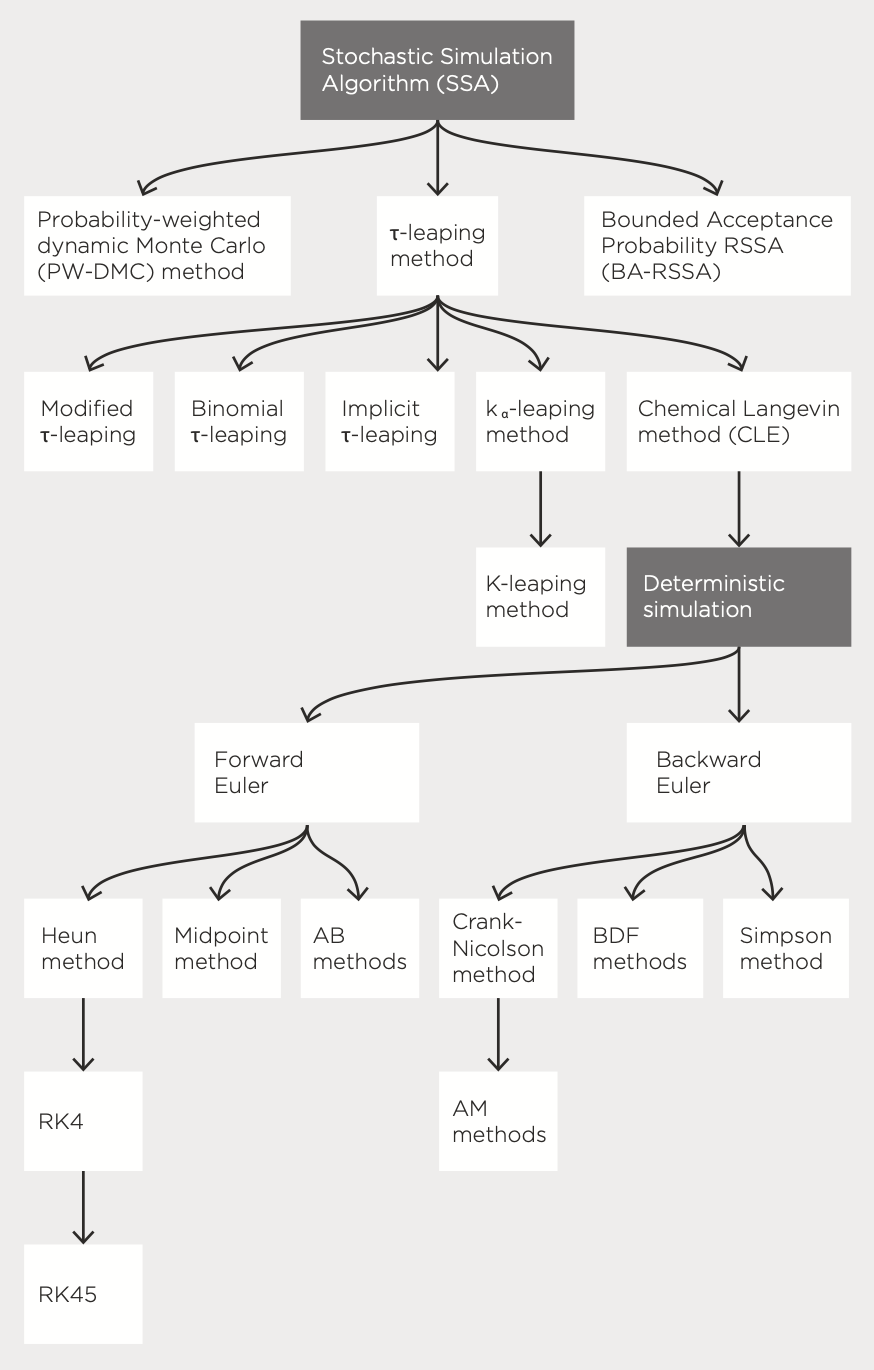
\includegraphics[width=\textwidth]{SSA_tree.png}
  \caption{Relationship between stochastic simulation algorithms}
    \label{fig:SSA_tree}
\end{figure}


To improve the exact simulations algorithms, one should consider to:

\begin{multicols}{2}
  \begin{itemize}
    \item Work on the number of reaction events, grouping them in such a way to reduce the number of reactions in the system.
      The $\tau$ leaping methodology is working in this direction.
    \item Improve the computation of the propensity.
      For instance, the probability-weighted Monte Carlo is particularly promising in situations in which there is a huge differences in propensities among reactions.
  \end{itemize}
\end{multicols}

\section{Probability-Weighted Dynamic Monte Carlo Method}
The probability-weighted dynamic Monte Carlo method (PW-DMC) is an approximation approach for improving the computational efficiency of stochastic simulations of reaction networks where some reactions have propensities significantly larger than other reactions.
This is because fast reactions (with large propensities) occur frequently and dominate the simulation, while slow reactions (with small propensities) occur less frequently.
The events from the slow reaction are rare and their statistical estimation is unreliable.
PW-DMC attempts to equalize the propensities of reactions so that a larger increment time step can be chosen, improving simulation's performance.

  \subsection{Weighted sampling}
  The principle of this algorithm is a sort of modification of the probability distribution of the next reaction firing through weighted sampling.
  The propensity $a_j$ of $R_j$ is scaled by a biasing weight $w_j$ defined as the number of firing of $R_j$ at each step.
  To compute it the unweighted probability $\frac{a_j}{a_0}$ is discretized into integer valued histogram bins according to a size $b$.

    \subsubsection{Effective propensity}
    The effective propensity $a^w_j$ is computed as:

    $$a^w_j = \frac{a_j}{w_j}$$

    These are then used for the selection of $R_\mu$.
    The chance that a slow reaction fires is increased and so is the frequency of rate events.

  \subsection{Realization of the reaction firing}
  The realization of the next reaction firing has two step:

  \begin{multicols}{2}
    \begin{itemize}
      \item Selection of the reaction.
      \item Correction of the firing time.
    \end{itemize}
  \end{multicols}

    \subsubsection{Selection of the reactoin}
    $R_\mu$ is selected with probability $\frac{a_\mu^w}{a_0^\mu}$, where $a_0^\mu = \sum\limits_{j=1}^Ma_j^w$.
    This can be done by linearly accumulating $a_\mu^w$ as:

    $$\mu = \arg\min\limits_{j\in \mu}\sum\limits_{j=1}^\mu a_j^w\ge r_1a_0^w$$

    Where $r_1\sim norm(0,1)$.

    \subsubsection{Correction of the firing time}
    The firing time $\tau$ is corrected to account for the bias.
    $\tau$ is generated from an exponential distribution with rate $a_0^w$:

    $$\tau = \frac{1}{a_0^w}\ln\left(\frac{1}{r_2}\right)$$

    Where $r_2\sim norm(0,1)$.
    Then the state at time $t+\tau$ is updated assuming there are $w_\mu$ consecutive firings of $R_\mu$ in $[t,t+\tau[$ ant the state at time $t+\tau$ is updated as:

    $$X(t+\tau) = X(t) + w_\mu\vec{v}_\mu$$

    The weight of the reactions have to be updated accordingly.

  \subsection{Bounds on the weights}
  $w_j$ should be an integer value because the population of a species involved in a reaction is an integer.
  Its magnitude is constrained in order to bound the error in the results.
  Each time $R_j$ is selected it fires $w_j$ times.
  The change of each species $S_i$ in $R_j$ is $w_j$, the fluctuation of the population is thus $\frac{w_j}{X}$.
  This ratio must be less than a predefined tolerance $\epsilon$ to ensure the statistical uncertainty of the estimation of $X_i$.
  Moreover the ration would be negligibly small when the population of species is large, and the chosen weight does not affect the simulation result.
  However the weight introduces an approximation to the temporal dynamics when the population of species is low and in this case $w_j$ must be adjusted to maintain $w_j< \epsilon X_i$.

  \subsection{Algorithm}
  An implementation of PW-DMC can be found in algorithm \ref{algo:pw-dmc}.

  \begin{algorithm}[H]
\DontPrintSemicolon
\SetKwComment{comment}{$\%$}{}
\SetKw{Int}{int}
\SetKw{To}{to}
\SetKw{Return}{return}
\SetKw{Not}{not}
\SetKw{Input}{Input}
\SetKw{Output}{Output}
\SetKwData{Item}{item}
\SetKwFunction{Min}{min}
\SetKwFunction{TitleFunction}{Probability-Weighted Dynamic Monte Carlo (PW-DMC)}

\caption{\protect\TitleFunction{}}
\label{algo:pw-dmc}

\Input: a biochemical reaction network of $M$ reactions in which each reaction $R_j$, $j=1, \dots, M$ is accompanied with the state change vector $\vec{v}_j$ and the propensity $a_j$, the initial state $\vec{x}_0$ at time $0$ and the simulation ending time $T_{\max}$, the size $b$ for discretizing probability of reacitons and tolerance $\epsilon$ for constraining the fluctuation of species.\;

\Output: a trajectory of the biochemical reaction network, which is a collection of states $X(t)$ for time $0\le t\le T_{\max}$\;

$t = 0$\;
$\vec{X} = \vec{x}_0$\;
build the reaction dependency graph $G$\;
compute propensity $a_j$ for each reaction $R_j$\;

\While{$t<T_{\max}$}{
	compute $w_j$ for each $R_j$\;
	compute $a_j^w = \frac{a_j}{w_j}$ for each $R_j$\;
	$a_0^w = \sum\limits_{j=1}^Ma_j^w$\;
	generate two random numbers $r_1, r_2\sim norm(0,1)$\;
	select $R_\mu$ with the smallest index $\mu$ such that $\sum\limits_{j=1}^\mu a^w_j\ge r_1a^w_0$\;
	$\tau = \frac{1}{a^w_0}\ln\frac{1}{r_2}$\;
	$\vec{X} = \vec{X}+w_\mu\vec{v}_\mu$\;
	$t=t+\tau$\;
	\ForEach{$R_j\in Dependents(R_\mu)$}{
		update $a_j$\;
	}
}

\end{algorithm}


  \subsection{Discussion}

    \subsubsection{Time complexity}
    The speed-up gain in PW-DM is achieved by multiple firings of a reaction in each step.
    The weight can be tuned to produce a significant gain in computational performance, while keeping accuracy.
    The frequency of rare events is increased, helping explore more the biochemical systems.

    \subsubsection{Limitations}
    PW-DMC skews the probability distribution of the state, because the weight sampling groups reaction of the same type in bundles and fires them together, loosing the order of reaction.
    PW-DMC could misdescribe the fluctuation of species in the result.
    $\epsilon$ has to be set for constraining fluctuation of species to a reasonably small value in order to bound the accuracy of the simulation.

\section{Bounded acceptance probability RSSA}
The bounded acceptance probability RSSA BA-RSSA focuses on the simulation of reactions involved species with both small and large population.
These will have a large propensity.
Many firings can occur in time interval and quickly deplete the small population species.
To bound the error updates must be performed frequently, degrading the simulation performance, especially if the small population is a hub species.
The simulation of this reactions is accelerated by bounding the acceptance of a candidate reaction selected by RSSA.
It accepts a candidate reaction without validation if its acceptance probability is greater than a user-defined probability, reducing the computational cost for both selecting of reaction firing and propensity updates.

  \subsection{Defining the bounds}
  Let $0\le\alpha\le 1$ be a constant defined as a lower bound for the acceptance probability and $R_j$ the selected reaction.
  BA-RSSA guarantees that the probability that $R_j$ is accepted to fire is greater than $\alpha$.
  The validation step of standard RSSA accepts $R_j$ to fire with probability $\frac{a_j(X(t))}{\overline{a_j}}$, the goal of BA-RSSA is to ensure:

  $$\frac{a_j(X(t))}{\overline{a_j}} \ge \alpha$$

  This is difficult to assess because it depends on $X(t)$.
  Anytime the state changes $a_j$ has to be re-evaluated.
  To cope with this BA-RSSA exploits the fact that $a_j(X(t))\ge \underline{a_j}$ when $X(t)\in[\underline{X}, \overline{X}]$, therefore if:

  $$\frac{\underline{a_j}}{\overline{a_j}}\ge \alpha$$

  Holds for each reaction $\frac{a_j(X(t))}{\overline{a_j}} \ge\alpha$ is automatically satisfied.

  \subsection{Defining the fluctuation interval}
  To enforce $\frac{\underline{a_j}}{\overline{a_j}}\ge \alpha$, $[\underline{X}, \overline{X}]$ has to be defined so that $\frac{\underline{a_j}}{\overline{a_j}}$ of each $R_j$ within the fluctuation interval is bounded by $\alpha$.
  A fluctuation rate $\delta_i$ for each $S_i$ involved in $R_j$ has to be selected so that when $S_i$ fluctuates in $[(1-\delta_i)X_i(t), (1+\delta_i)X_i(t)]$ the inequality is satisfied.
  Only a range of $\delta_i$ can be chosen given the ratio of propensity bounds.

    \subsubsection{Computing the maximum fluctuation rate}
    The maximum fluctuation rate $\delta_i$ computation is reaction dependent.

      \paragraph{Synthesis reaction}
      For a synthesis reaction $R_j$, $a_j$ is independent of $X(t)$ and is equal to $x_j$.
      Also the bounds are constant, the ratio is equal to $1$ and the inequality is satisfied.

      \paragraph{Unimolecolar reaction}
      For a unimolecular reaction $R_j$, $\overline{a_j} = c_j(1+\delta_i)X_i$ and $\underline{a_j} = c_j(1-\delta_i)X_i$, so that the inequality becomes:

      $$\frac{1-\delta_i}{1+\delta_i}\ge\alpha$$

      The maximum value of $\delta_i$ then becomes:

      $$\delta_i = \frac{1-\alpha}{1+\alpha}$$

      \paragraph{Bimolecular reaction}
      For a bimolecular reaction $R_j$ $\overline{a_j} = c_j(1+\delta_j)(1+\delta_k)X_iX_k$ and $\underline{a_j} = c_j(1-\delta_i)(1-\delta_k)X_iX_k$, so that:

      $$\frac{(1-\delta_i)(1-\delta_k)}{(1+\delta_i)(1+\delta_k)}\ge \alpha$$

      Which is a quadratic equation of two independent variables, which can be splitted in to part so that:

      $$\frac{1-\delta_i}{1+\delta_i}\ge\sqrt{\alpha}\land\frac{1-\delta_k}{1+\delta_k}\ge\sqrt{\alpha}$$

      So that the maximum values for the fluctuation rates are:

      $$\delta_i = \delta_k = \frac{1-\sqrt{\alpha}}{1+\sqrt{\alpha}}$$

      \paragraph{Dimerization reaction}
      For a dimerization reaction $R_j$ by a similar derivation as the bimolecular one:

      $$\frac{(1-\delta_i)((1-\delta_i)X_i-1)}{(1+\delta_i)((1+\delta_i)X_i-1)}\ge\alpha$$

      So that the maximum $\delta_i$:

      $$\delta_i = \frac{1-\sqrt{\alpha}}{1+\sqrt{\alpha}}\left(1-\frac{1}{X_i}\right)$$

  \subsection{Selecting the propensity}
  Once the state is confined in a fluctuation interval that satisfies the bounds, any $b_j\in[\underline{a_j}, \overline{a_j}]$ can be chosen as the propensity.
  The extreme values may bias the selection step, so the average can be used:

  $$b_j = \frac{\underline{a_j}+\overline{a_j}}{2}$$

  This choice requires two evaluation of the propensity function.
  Another choice is to compute the value of the propensity at the central point of the fluctuation interval so to have one evaluation of the propensity function:

  $$b_J = a_j\left(\frac{\underline{X}+\overline{X}}{2}\right) = a_j(X(t))$$

  \subsection{Algorithm}
  An implementation of BA-RSSA can be found in algorithm \ref{algo:ba-rssa}.

  \begin{algorithm}[H]
\DontPrintSemicolon
\SetKwComment{comment}{$\%$}{}
\SetKw{Int}{int}
\SetKw{To}{to}
\SetKw{Return}{return}
\SetKw{Not}{not}
\SetKw{Input}{Input}
\SetKw{Output}{Output}
\SetKw{False}{false}
\SetKw{True}{true}
\SetKwData{Item}{item}
\SetKwFunction{Min}{min}
\SetKwFunction{TitleFunction}{Buonded Acceptance Probability RSSA (BA-RSSA)}

\caption{\protect\TitleFunction{}}
\label{algo:ba-rssa}

\Input: a biochemical reaction network of $M$ reactions in which each reaction $R_j$, $j=1, \dots, M$ is accompanied with the state change vector $\vec{v}_j$ and the propensity $a_j$, the initial state $\vec{x}_0$ at time $0$ and the simulation ending time $T_{\max}$ and the bon=und of the acceptance probability $0\le\alpha\le 1$\;

\Output: a trajectory of the biochemical reaction network, which is a collection of states $X(t)$ for time $0\le t\le T_{\max}$\;

$t = 0$\;
$\vec{X} = \vec{x}_0$\;
build the species reaction SR dependency graph $\mathcal{G}$\;
define $\delta_i\forall S_i$ involved in $R_j$ to ensure that the acceptance of $R_j$ is bounded by $\alpha$\;
compute the fluctuation interval $[\underline{X_i}, \overline{X_i}] = [(1-\delta-i)X_i, (1+\delta_i)(X_i)]$ for each species $S_i$ around its current population $X_i$\;
compute $b_j$ for each $R_j$\;
$b_0 = \sum\limits_{j=1}^Mb_j$\;
$\overline{a_0} = 0$\;

\ForEach{$R_j\in$ Reactions}{
	compute $\overline{a_j}$ and $\underline{a_j}$\;
	$\overline{a_0} = \overline{a_0} + \overline{a_j}$\;
}

\While{$t<T_{\max}$}{
	\Repeat{$\exists(X_i\not\in[\underline{X_i},\overline{X_i}])$}{
		generate two random numbers $r_1, r_2\sim norm(0,1)$\;
		select minimum index $\mu$ such that $\sum\limits_{j=1}^\mu b_\mu\ge r_1b_0$\;
		$\tau = \frac{1}{b_0}\ln(r_2)$\;
		$\vec{X} = \vec{X}+\vec{v}_\mu$\;
		$t=t+\tau$\;
	}
	\ForEach{$X_i\not\in[\underline{X_i}, \overline{X_i}]$}{
		define a new $[\underline{X_i}, \overline{X_i}] = [(1-\delta-i)X_i, (1+\delta_i)(X_i)]$\;
		\ForEach{$R_j\in ReactionsAffectedBy(S_i)$}{
			update $b_j$ and $b_0$\;
		}
	}
}
\end{algorithm}


  \subsection{Discussion}
  When $\alpha = 1$ return to the exact case.

    \subsubsection{Time complexity}
    BA-RSSA reduces the selection cost for the next reaction firing and avoids a large number of the propensity updates.
    The selected reaction firing is ensured to fire with  probability greater than a threshold when the population is confined in its fluctuation interval.
    The propensity updates are performed infrequently and only locally.


\section{$\mathbf{\tau}$-Leaping method}
The aim of the $\tau$-leaping method is to discretize the time axis into intervals and to approximate the number of reaction firing in each one.
The simulation then leaps form one interval to the next with many reaction firing performed simultaneously.

  \subsection{Simulation time}
  The simulation time is discretized into







\section{\texorpdfstring{$\tau$-Leaping Method}{-Leaping Method}}
The $\tau$-leaping method is a stochastic approximate algorithm for improving performance of stochastic simulation.
Its aim is to discretize the time axis into time intervals and to approximate the number of reactions firing in each time interval.
The simulation then leaps from one time interval to the next interval with many reaction firings performed simultaneously.
What is remarkable here, is that we are doing an approximation over the number of iterations which is much more relevant than previous approaches.
We are grouping a mixture of events, which can be defined as a \emph{macrostep}.
If $\tau$ is big, the number of iterations will be low and the complexity will decrease.
We should constraint the error in such a way that we are aware of its value as a constant.
Which could be a high-level property of tau to apply macrostep without a crude error in the simulation? We should impose certain logics on $\tau$.
\\
\\
\noindent
We want to limit the bias on the propensity.
This translates in tau selection satisfying the so-called ``\textbf{leap condition}'':
\\
\\
\noindent
There exists a leap $\tau > 0$ such that the change in propensity $a_j$ of each reaction $R_j$ with $j = 1,...,M$ during the time interval $[t,t +\tau)$ is negligibly small.
Negligibly small means lower than some threshold.
\\
\\
\noindent
By applying a proper reasoning we reach the following formula, in which we derive the update of the state.
Once we have selected $\tau$, we will evolve the system by adding to he current state a certain amount of firing for each one of the reactions in the system {[}for each reaction j from 1 to m we apply a certain amount of time{]}.
$$ X(t+\tau)=\mathbf{x}+\sum_{j=1}^{M}k_j\mathbf{v}_j =\mathbf{x}+\sum_{j=1}^{M}Poi(a_j(x)\tau)\mathbf{v}_j $$
$k_j$ will be generated through a Poisson distribution, which will depend over the specific propensity multiplied by the size of the step.
The algorithm is applying any of the reactions per a specific amount of time.
\begin{itemize}
\item Pros: we are allowed to work with higher $\tau$ with respect to exact stochastic simulations.
\item Cons: if we only have rare events, the algorithm will not be the best solution (as it will try to apply all reactions at all the times).
\end{itemize}
\noindent
Given however that in any system there are at least some reactions with high propensity, at the very end we still gain a huge speed-up.

\subsection{Choosing tau - Leap selection section}

\subsubsection{Postleap Selection}
Choose a $\tau$ from a Poisson distribution and see if it is fine for the simulation.
We start from a predefined arbitrary $\tau$ (small), then we have a trial procedure.
The algorithm will compare the difference in the propensity before and after, to assess whether $\tau$ is of the right size.
E.g. if the change in propensity is small, we can use a greater $\tau$.
The complexity of the $\tau$-leaping is moved to a sub-problem, which is the choice of $\tau$ .
We could also perform a preleap selection or choose other strategies.
The Poisson distribution could provide more events than the ones that are possible in the system; in this case we end up with a negative population.
While performing $\tau$-leaping, we will need to make sure that a negative scenario is never reached through a test.
The real amount of time executing k should be computed as the mean from k generated from Poisson distribution and the availability of the reactants {[}non chiaro{]}.
We can bridge $\tau$-leaping with exact stochastic simulation when we have only rare events.

\section{Chemical Langevin Method}
We can use the Normal distribution instead of Poisson, and scale it with mean and variance with another Normal formula based on a (0,1) distribution, obtaining a simplified method.
We will not have main events, but main \emph{drivers} in the system.
Stochasticity is strongly approximated, we are moving to an idea of average, real numbers.
This will be the starting point for the deterministic simulation.
\\
\\
\noindent
\textbf{COPASI} is a well-known simulator.
It exploits Gillespie's algorithm and $\tau$-leaping algorithm.
In general, any simulator offers many algorithms, so we should be able to choose the best computational approach → calibrating the model.
The stochastic rate provides us the speed, we require to derive it with some methods; all simulations algorithm compute deterministically or stochastically a speed for the reaction, computed over parameters of the model e.g.~the rates.
The rates, as the initial values, are not free-lunch, they can be derived through experiments.
Often times, we work with models with not fully known parameters; in the second module we will explore solutions for \emph{estimating the parameters} (reverse engineering approach).
\\
\\
\noindent
\textbf{\emph{Adaptive algorithms}} select a delta and change it adaptively during the simulation in order to reach the best results, for instance post leap $\tau$ selection.
\textbf{Chemical Langevin Method} allows to modify the evolution of the system; the update formula depends on the propensity, but allows to distinguish a totally deterministic part from the stochastic one.
This algorithm also has an important difference with previously seen strategies: we do not have integers, we will be provided with a real number adding some noise.
This dynamics is over continuous numbers, tends to an average behaviour.
